\documentclass[journal,onecolumn]{IEEEtran}
\usepackage{graphicx}
\usepackage{booktabs}
\usepackage{multirow}
\usepackage{float}
\usepackage{placeins}
\usepackage{amsmath}
\usepackage{amssymb}

\graphicspath{{./images/}}

\begin{document}

\title{Supplementary Materials for\\
ADMET-Bench: Task-Dependent Performance of GNNs and Pretrained Models in ADMET Prediction}

\author{}

\maketitle

\renewcommand{\thetable}{S\arabic{table}}
\renewcommand{\thefigure}{S\arabic{figure}}

\section{Architecture-Selection Experiments}
\label{sec:supp_architecture}

This supplementary document reports the preliminary architecture-selection screen used to choose the graph neural network backbone for the main study. Eight message-passing variants (GraphConv, GCN, GAT, GraphSAGE, GIN, TAG, SGC, and TransformerConv) were evaluated on all six benchmark endpoints under the \emph{same} scaffold-split pipeline, target transformations, and evaluation metrics used in the main manuscript. For each architecture and endpoint the reported result is the best of five configurations selected on the validation split (searching over hidden dimension, number of layers, and learning rate), giving $8 \times 6 \times 5 = 240$ training runs in total. Because the screen shares the main study's protocol, the values below are directly comparable to the main-text results; they are provided for transparency and reproducibility and, as discussed in the main text, show that no single architecture dominates across endpoints.

\begin{table}[H]
\centering
\caption{Preliminary classification architecture screen: each architecture is evaluated at its best of five configurations selected on the validation split (search over hidden dimension, number of layers, and learning rate). Test AUC-ROC and F1 on the scaffold-split test set. Best AUC per task in \textbf{bold}.}
\label{tab:arch_classification}
\small
\setlength{\tabcolsep}{4pt}
\begin{tabular}{lcccc}
\toprule
\textbf{Architecture} & \multicolumn{2}{c}{\textbf{Tox21 (NR-AR)}} & \multicolumn{2}{c}{\textbf{hERG}} \\
 & \textbf{AUC} & \textbf{F1} & \textbf{AUC} & \textbf{F1} \\
\midrule
GraphConv & 0.741 & 0.495 & 0.775 & 0.784 \\
GCN & \textbf{0.755} & 0.345 & 0.732 & 0.829 \\
GAT & 0.695 & 0.419 & 0.725 & 0.725 \\
GraphSAGE & 0.711 & 0.329 & 0.785 & 0.863 \\
GIN & 0.724 & 0.481 & 0.733 & 0.841 \\
TAG & 0.726 & 0.247 & 0.765 & 0.813 \\
SGC & 0.708 & 0.409 & \textbf{0.795} & 0.892 \\
Transformer & 0.726 & 0.466 & 0.734 & 0.856 \\
\bottomrule
\end{tabular}
\end{table}

\begin{table}[H]
\centering
\caption{Regression architecture screen: average rank across the four ADME regression datasets (by test R$^2$, lower rank is better); each architecture is evaluated at its best of five configurations selected on the validation split (search over hidden dimension, number of layers, and learning rate). Per-dataset test R$^2$ shown for reference. GraphConv (deployed backbone) in \textbf{bold}.}
\label{tab:arch_regression}
\small
\setlength{\tabcolsep}{4pt}
\begin{tabular}{lccccccc}
\toprule
\textbf{Arch.} & \textbf{Avg Rank} & \textbf{Caco-2} & \textbf{Half-Life} & \textbf{Clear. Hep.} & \textbf{Clear. Mic.} & \textbf{Params} & \textbf{Time (s)} \\
\midrule
GCN & 3.25 & 0.480 & 0.259 & $-$2.039 & 0.227 & 463k & 9.0 \\
Transformer & 3.25 & 0.459 & 0.279 & $-$0.835 & 0.139 & 987k & 12.6 \\
TAG & 4.00 & 0.471 & 0.076 & $-$0.483 & $-$0.494 & 846k & 11.9 \\
\textbf{GraphConv} & 4.75 & 0.443 & $-$0.044 & $-$0.018 & $-$1.911 & 81k & 8.9 \\
SGC & 4.75 & 0.380 & 0.207 & $-$0.144 & $-$0.738 & 180k & 9.4 \\
GAT & 4.75 & 0.368 & 0.288 & $-$1.012 & 0.083 & 145k & 12.8 \\
GIN & 5.00 & 0.487 & $-$0.054 & $-$0.655 & $-$10.000 & 726k & 8.5 \\
GraphSAGE & 6.25 & 0.442 & $-$0.296 & $-$2.660 & 0.133 & 247k & 9.0 \\
\bottomrule
\end{tabular}
\end{table}

The classification screen (Table~\ref{tab:arch_classification}) shows that several architectures are competitive on the two toxicity endpoints: on Tox21 (NR-AR) the eight backbones span AUC $=0.695$--$0.755$, with GraphConv second best (0.741) behind GCN (0.755); on hERG they span AUC $=0.725$--$0.795$, with GraphConv at 0.775. The regression screen (Table~\ref{tab:arch_regression}) confirms that no architecture dominates: GraphConv attains a competitive Caco-2 R$^2$ (0.443) while, like every other backbone, collapsing to large negative R$^2$ on the weakly-learnable clearance and half-life endpoints (e.g., GCN $-2.04$ on hepatocyte clearance, GIN $-10.0$ on microsomal clearance, GraphSAGE $-2.66$ on hepatocyte clearance). This instability is a property of the endpoints rather than of any single backbone. GraphConv was selected as the shared backbone because it remains competitive on the learnable endpoints while using only $\approx$81k parameters—$5$--$12\times$ fewer than GCN (463k) or TransformerConv (987k)—and is among the fastest to train.

\begin{figure}[H]
    \centering
    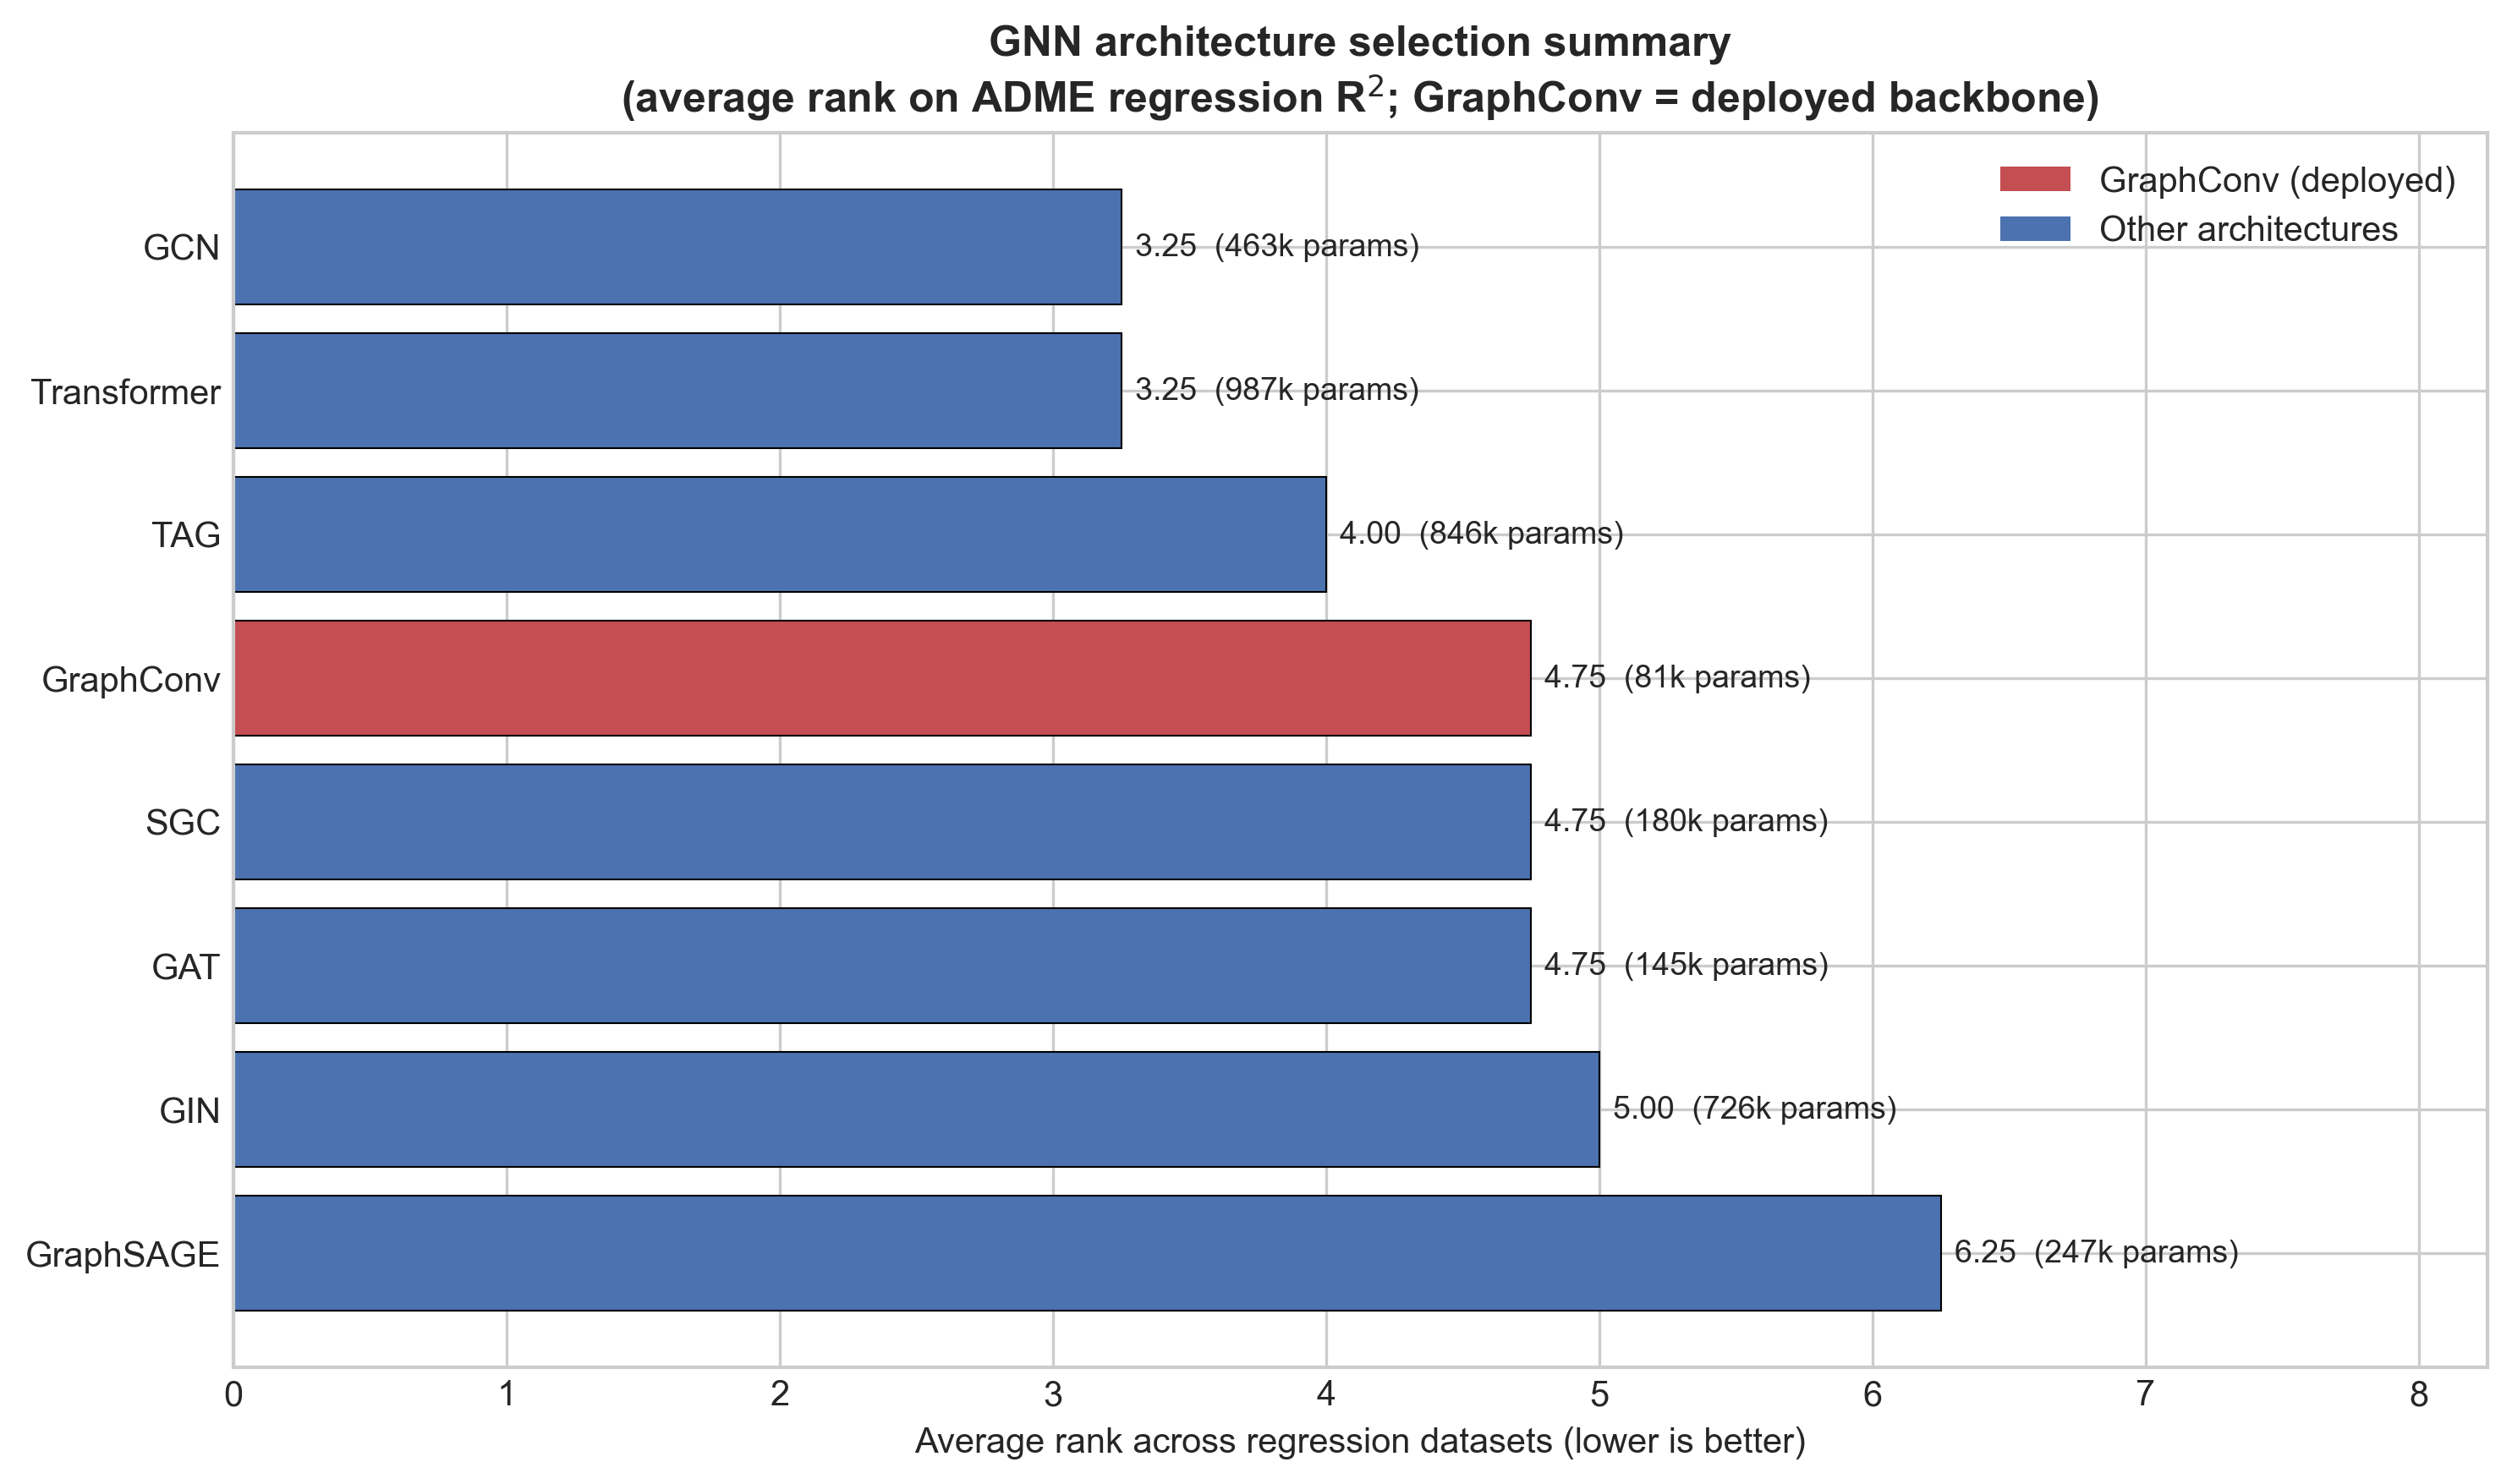
\includegraphics[width=0.95\textwidth,height=0.30\textheight,keepaspectratio]{arch_selection_summary.png}
    \caption{Preliminary architecture-selection summary showing average rank across the regression datasets (lower is better), colored by training stability. GraphConv was selected based on its combination of competitive performance, parameter efficiency, and runtime efficiency.}
    \label{fig:arch_selection_summary}
\end{figure}

\begin{figure}[H]
    \centering
    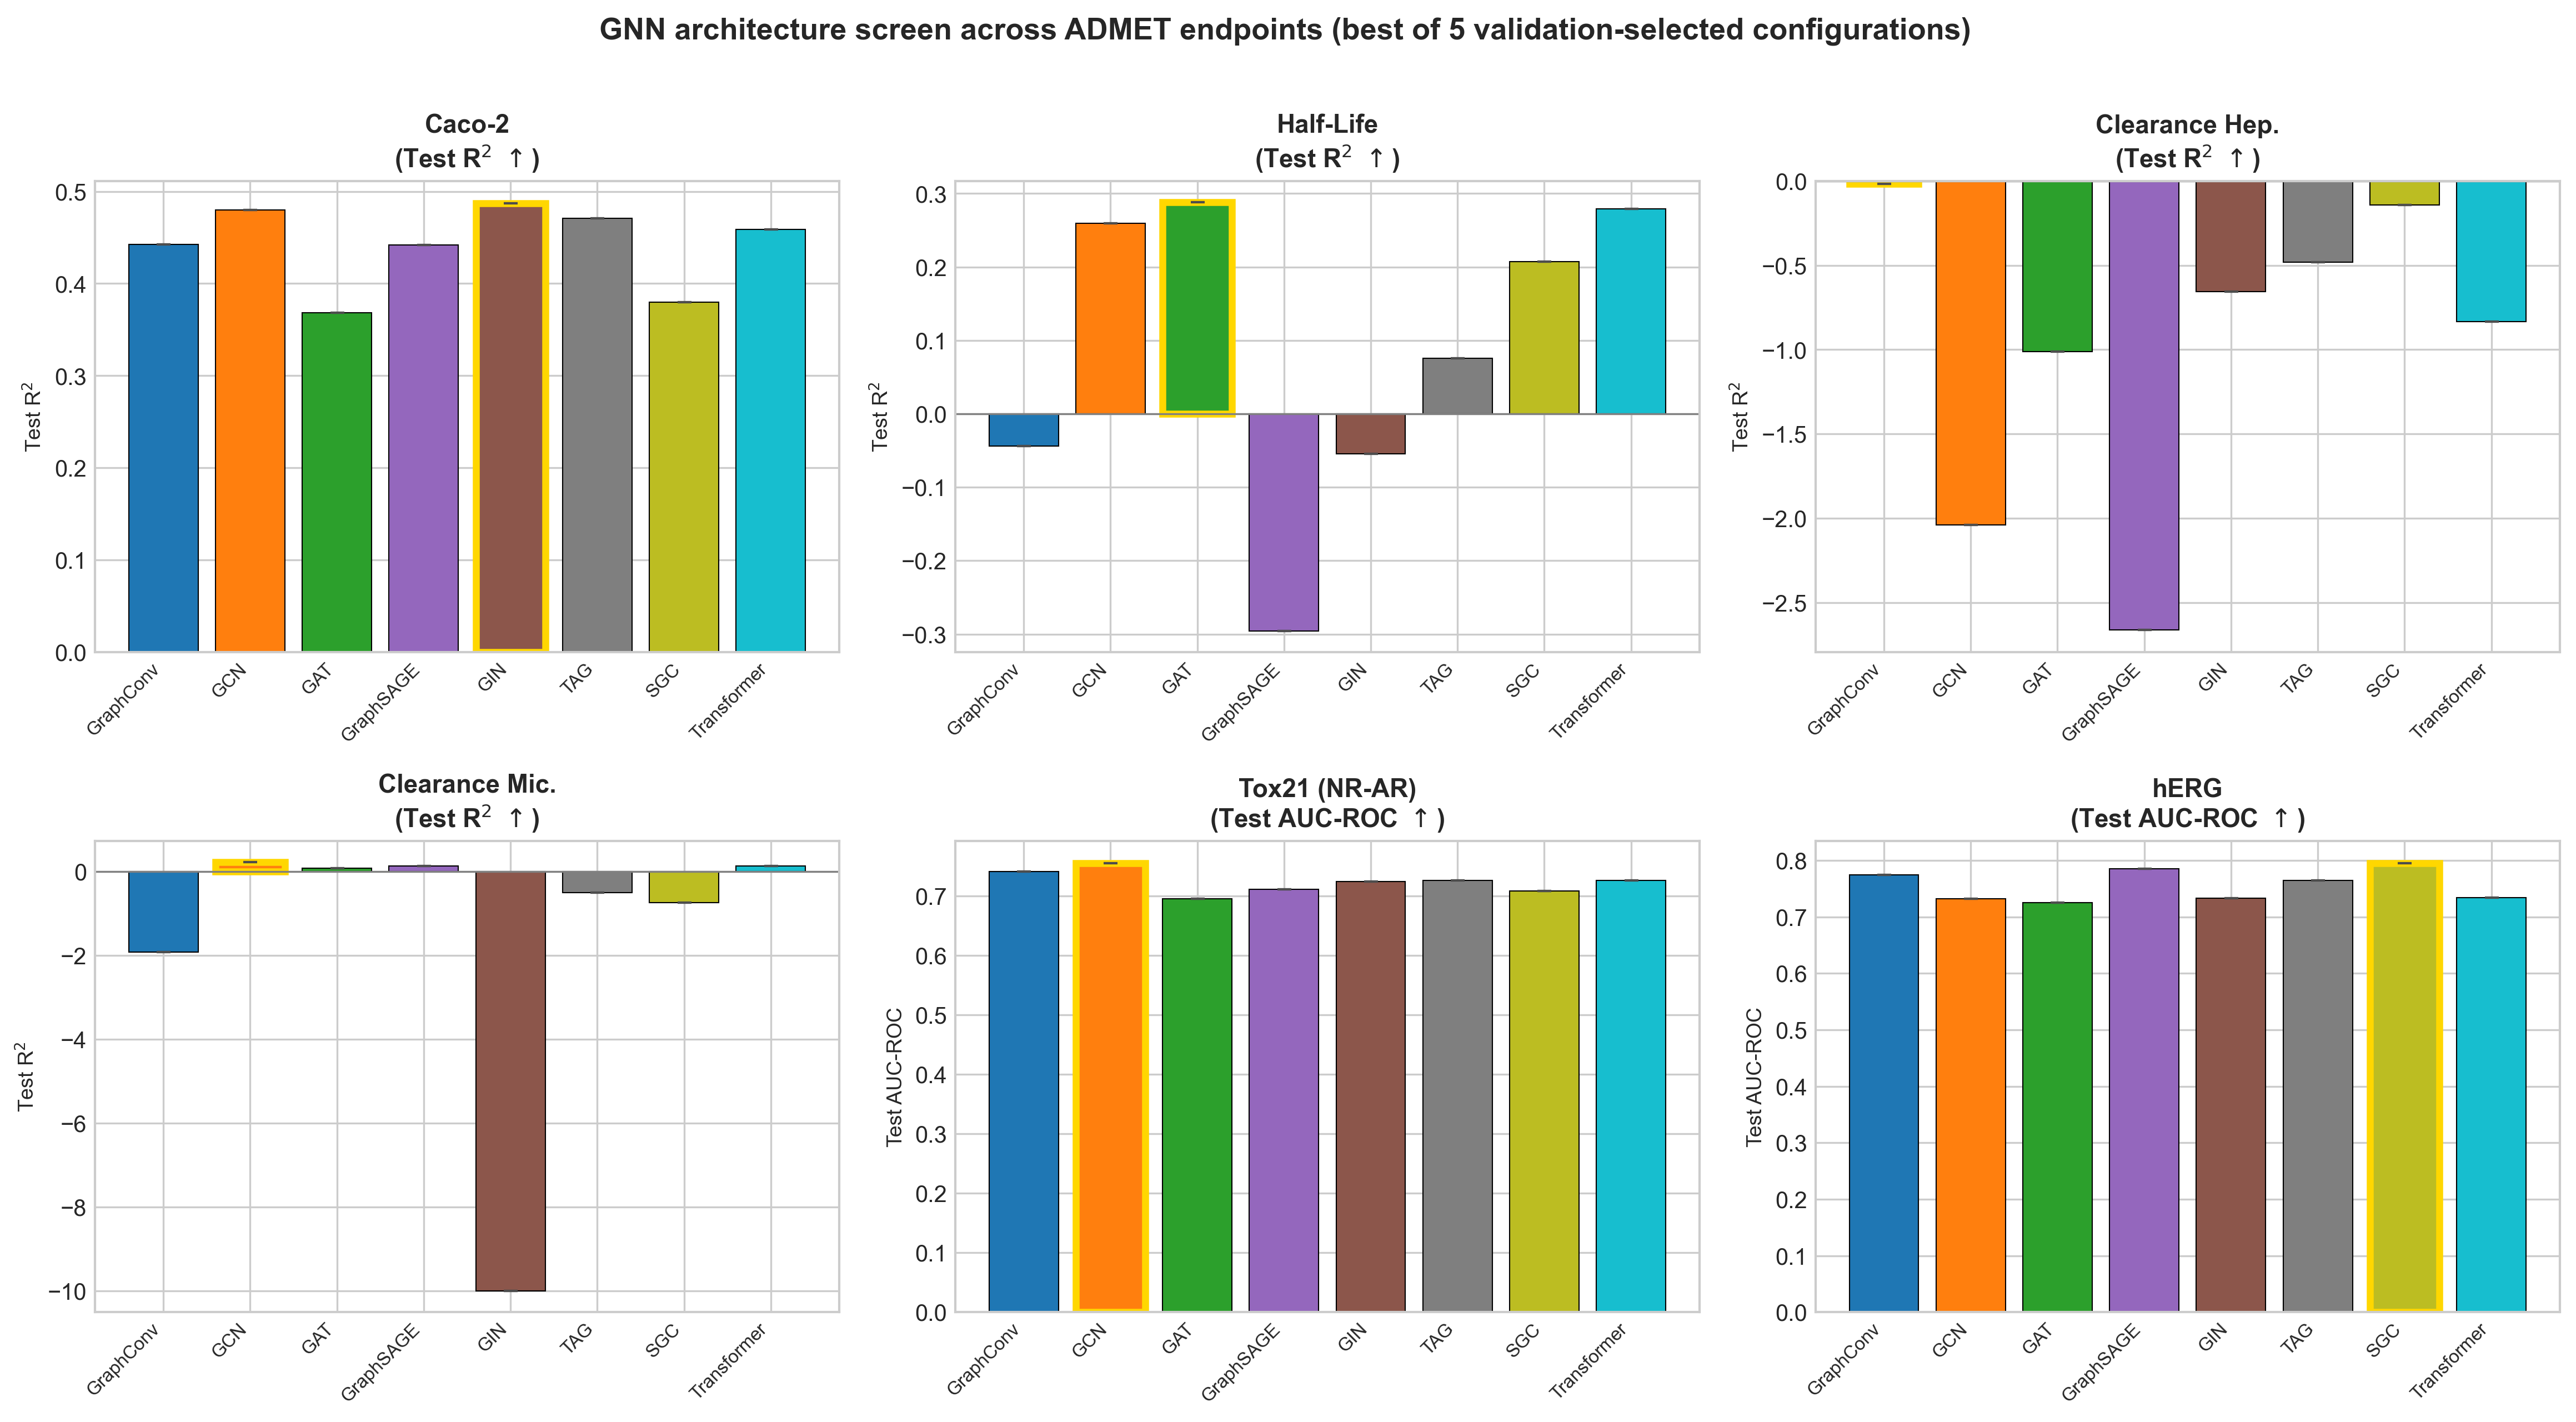
\includegraphics[width=0.95\textwidth,height=0.42\textheight,keepaspectratio]{arch_comparison_all_datasets.png}
    \caption{Per-dataset architecture comparison across all six benchmark endpoints. Classification endpoints (Tox21, hERG) are shown by test AUC-ROC and regression endpoints (Caco-2, Half-Life, Hepatocyte and Microsomal Clearance) by test R$^2$. The weakly-learnable clearance and half-life endpoints are unstable across all eight architectures, whereas the structure-driven endpoints cluster within a narrow band.}
    \label{fig:arch_comparison}
\end{figure}

\end{document}
